\documentclass{article}

\usepackage{xcolor}
\usepackage{tikz}
\usetikzlibrary{trees}
\usepackage[utf8]{inputenc}
\usepackage{amsmath}
\usepackage{enumerate}
\usepackage{microtype}
\usepackage[top=1.5cm]{geometry} % controls page margins

\title{Examen Parcial 1}
\author{Programación III \\ Facultad de Ingenierías - Universidad Tecnológica de Pereira \\ Ingeniería de Sistemas y Computación}
\date{Marzo 12 2026}
\begin{document}
\maketitle
\thispagestyle{empty}

\textbf{1. (1.5)} Definir el predicado \texttt{product\_digits/2} donde \texttt{product\_digits(N, P)} es verdadero si \texttt{P} es el producto de los dígitos de \texttt{N}. \newline \newline

\textbf{2. (1.0)} Considere el siguiente árbol genealógico:

\begin{center}
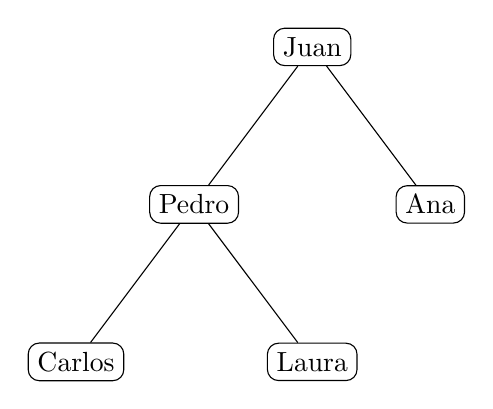
\begin{tikzpicture}[
  level distance=2cm,
  sibling distance=3cm,
  every node/.style={draw, rectangle, rounded corners}
]

\node {Juan}
    child { node {Pedro}
        child { node {Carlos} }
        child { node {Laura} }
    }
    child { node {Ana} };

\end{tikzpicture}
\end{center}

\textbf{a. } Escribir la base de conocimiento en prolog utilizando hechos para representar las relaciones de parentezco.

\textbf{b. } Definir un predicado \texttt{abuelo/2} donde \texttt{abuelo(X, Y).} es verdadero si \texttt{X} es el abuelo de \texttt{Y}. \newline \newline


\textbf{3. (2.5)} Escribir un predicado \texttt{fizzbuzz/2} que genere la secuencia FizzBuzz desde 1 hasta un número entero positivo \texttt{N}, donde \texttt{fizzbuzz(N, Resultado).} es verdadero si
\texttt{Resultado} es una lista de longitud \texttt{N} que contiene el valor correspondiente para cada número \texttt{i} desde \texttt{1} hasta \texttt{N}. \newline

Para cada posición \texttt{i} en la lista: 

\begin{itemize}
  \item Si \texttt{i} es divisible por \texttt{3} y \texttt{5}, el elemento debe ser \texttt{"FizzBuzz"}.
  \item Si \texttt{i} es divisible solo por \texttt{3}, el elemento debe ser \texttt{"Fizz"}.
  \item Si \texttt{i} es divisible solo por \texttt{5}, el elemento debe ser \texttt{"Buzz"}.
\end{itemize}

En cualquier otro caso, el elemento debe ser el número \texttt{i}. \newline

Ejemplo de consulta:
\begin{verbatim}
    ?- fizzbuzz(15, R).
\end{verbatim}

Resultado esperado:
\begin{verbatim}
    R = [1, 2, "Fizz", 4, "Buzz", "Fizz", 7, 8, "Fizz", "Buzz",
     11, "Fizz", 13, 14, "FizzBuzz"].
\end{verbatim}




\end{document}